% !TEX root = main.tex
\section{Results and findings}
We will now present the results of our experiments, going through each one of the already presented measures.

\subsection{Regularity}
As we stated before, the regularity tells us whether the users tend to be regular while tapping the red balloon during the activity. Let us first consider the first one, \testfirst. In Figure~\ref{fig:reg1} we can see the plot of the means squared error (from now on referred as MSE) for the activity. As we can see some sessions are very irregular in the beginning but all of them tend to a very low MSE, meaning that all the users are becoming very regular after a few seconds of activity. Besides of the observation of the graph this result is also confirmed by a very low average MSE of 0.15.

\todo[inline]{Unit measures on graphs. Also remove or mark the average line.}

\begin{figure}[h!t]
\centering
	{\setlength{\fboxsep}{1.5pt}
	 \fbox{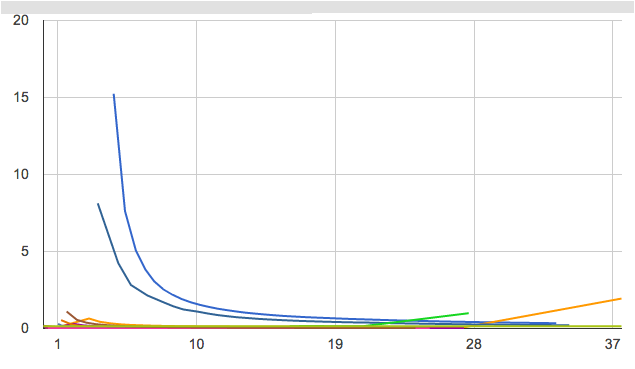
\includegraphics[width=0.45\textwidth]{reg1}}}
\caption{Regularity of \testfirst experiment}
\label{fig:reg1}
\end{figure}

On the other hand the MSE for the \testsecond experiment is very irregular, as shown in Figure~\ref{fig:reg2}, and does not tend to zero as the first one. We can observe that approximately for 5 seconds most of the users tend to tap regularly on the balloon, becoming then very irregular later on. This is probably due to the fact that during the first seconds of the activity they are trying to understand the balloon's behavior and when they get it they trying to inflate it as fast as they can, constantly increasing their tapping speed. This leads to very irregular tap intervals and a higher average MSE of 1.78.

\begin{figure}[h!t]
\centering
	{\setlength{\fboxsep}{1.5pt}
	 \fbox{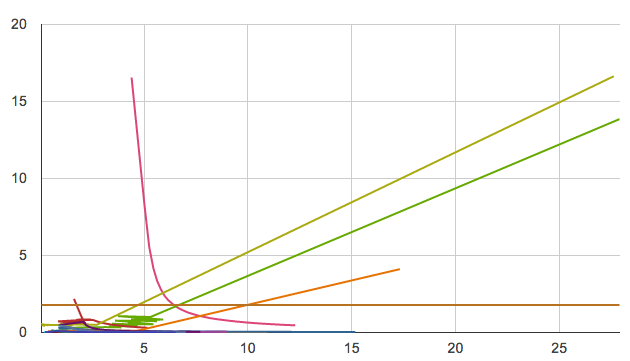
\includegraphics[width=0.45\textwidth]{reg2}}}
\caption{Regularity of \testsecond experiment}
\label{fig:reg2}
\end{figure}

\subsection{Synchronization}
We will now present the results about the synchronization score previously defined. Given the results of the regularity we would expect a priori a bad synchronization for the \testsecond experiment, given that having a good synchronization with irregular tap intervals would be possible only skipping random beats producing a tapping behavior which seems to be very uncommon.

As expected the synchronization score for the \testsecond experiment is pretty low, around 0.65. The \testfirst experiment on the other hand has a better sync score of 0.76, that, along with a consistent regularity, states a good synchronization of the users with the provided tempo.

As a further data we also observer that the number of taps for the first experiment had a very low variance of 0.53, with a mean of 46.08 taps. In fact the vast majority of the users (around 92\%) made exactly 46 taps, while only 2 users managed to tap 47 times. This confirms the good level of synchronization for such experiment, given the consistency of this result across all the users. The results are shown in Figure~\ref{fig:taps1}.

\begin{figure}[h!t]
\centering
	{\setlength{\fboxsep}{1.5pt}
	 \fbox{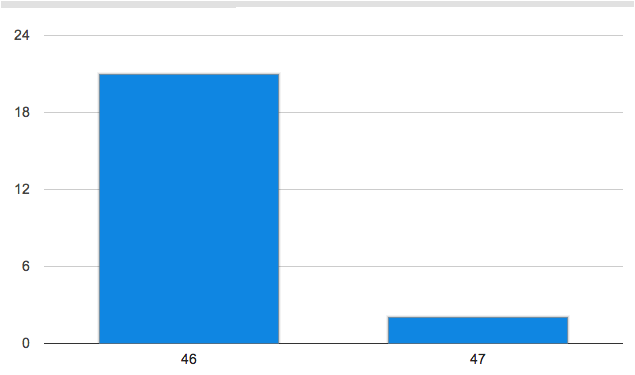
\includegraphics[width=0.45\textwidth]{nOfTaps1}}}
\caption{Number of taps distribution for the \testfirst experiment}
\label{fig:taps1}
\end{figure}

On the other hand the number of taps for the \testsecond experiment has a higher variance of 6.01, with a mean of 36.57 taps. Again this confirms that in such experiment every user had a different behavior, not being well synchronized with the background tempo. The results are shown in Figure~\ref{fig:taps2}.

\begin{figure}[h!t]
\centering
	{\setlength{\fboxsep}{1.5pt}
	 \fbox{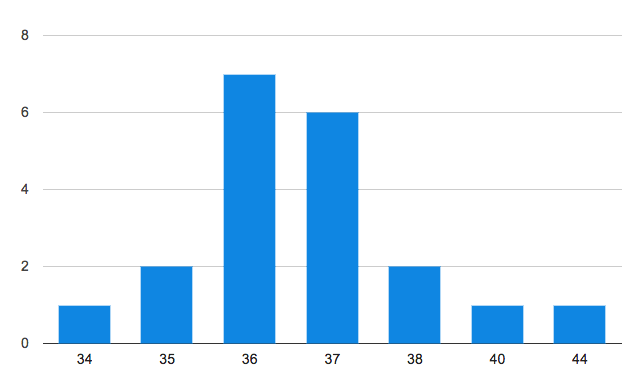
\includegraphics[width=0.45\textwidth]{nOfTaps2}}}
\caption{Number of taps distribution for the \testsecond experiment}
\label{fig:taps2}
\end{figure}

\subsection{Synchronization Ratio}
Finally we present the results of the synchronization ratio. Such measure was meant to be as a check in case of very poor synchronization score given a good regularity: in such a case there could have been the possibility that the user was still synchronizing, but with a tempo which was multiple (or divisor) of the given one.
Since this was not the case we expected the results to be consistent with the other measures and this was exactly the case.

In fact the synchronization ratio for the \testfirst experiment was 1.04, a result very close to 1, meaning that the user is synchronizing exactly on the given tempo.
For the \testsecond the synchronization ration was of 0.68, both far from the synchronization with the given tempo (1) and from the synchronization with half of the period (0.5).